\subsection{UMTS (3GSM)}
\selectlanguage{russian}

В третьем поколении сети GSM, называемом UMTS, защищённость немного улучшена. Общая схема аутентификации (рис.~\ref{fig:gsm3}) осталась примерно такой же, как и в GSM2. Жирным шрифтом на рисунке выделены новые добавленные элементы по сравнению с GSM2.
\begin{enumerate}
    \item Производится взаимная аутентификация SIM-карты и центра аутентификации по токенам $\textrm{RES}$ и $\MAC$.
    \item Добавлены проверка целостности и аутентификация данных (имитовставка\index{имитовставка}).
    \item Используются новые алгоритмы создания ключей, шифрования и имитовставки\index{имитовставка}.
    \item Добавлены счетчики на SIM-карте $\textrm{SQN}_\textrm{T}$ и в Центре аутентификации $\textrm{SQN}_\textrm{Ц}$ для защиты от атак воспроизведения. Значения увеличиваются при каждой попытке аутентификации и должны примерно совпадать.
    \item Увеличена длина ключа шифрования до 128 бит.
\end{enumerate}

\begin{figure}[!ht]
	\centering
	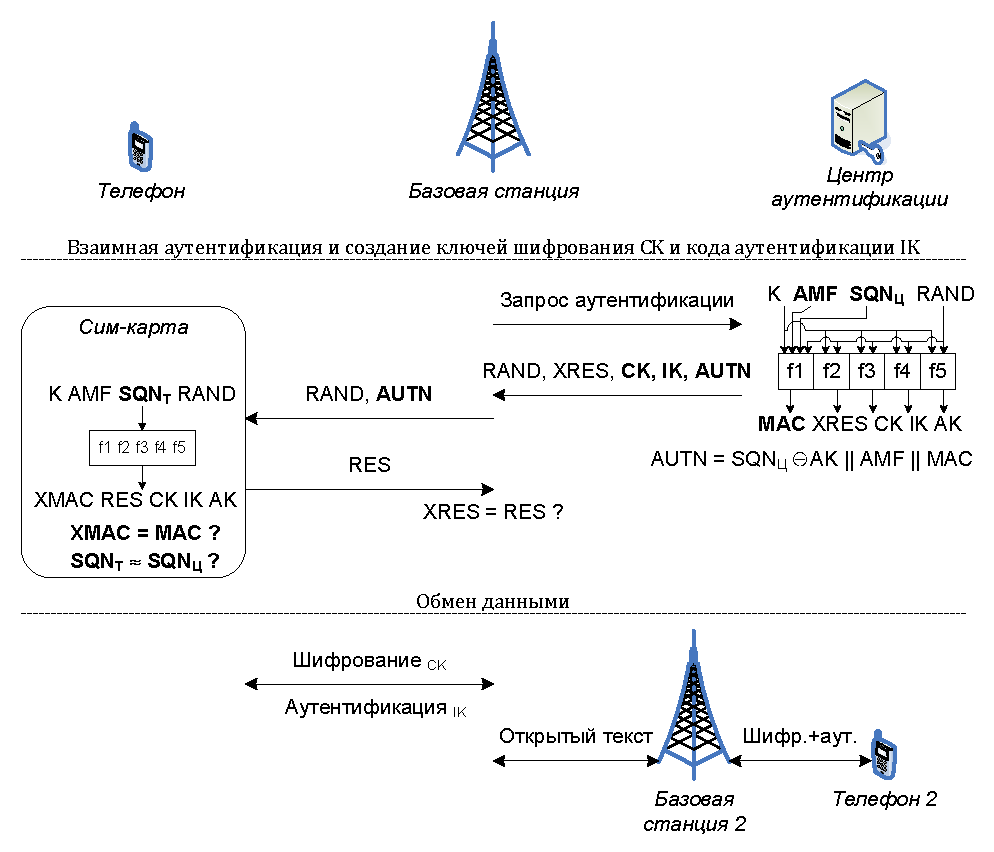
\includegraphics[width=\textwidth]{pic/gsm3}
	\caption{Взаимная аутентификация и шифрование в UMTS (3GSM)\label{fig:gsm3}}
\end{figure}

Обозначения на рис.~\ref{fig:gsm3} следующие:
\begin{itemize}
    \item $K$ -- общий секретный 128-битовый ключ SIM-карты и центра аутентификации.
    \item $\textrm{RAND}$ -- 128-битовое псевдослучайное число, создаваемое Центром аутентификации.
    \item $\textrm{SQN}_\textrm{T}, \textrm{SQN}_\textrm{Ц}$ -- 48-битовые счетчики для защиты от атак воспроизведения.
    \item $\textrm{AMF}$ -- 16-битовое значение окна для проверки синхронизации счетчиков.
    \item $CK, IK, AK$ -- 128-битовые ключи шифрования данных $CK$, кода аутентификации данных $IK$, гаммы значения счетчика $AK$.
    \item $\MAC, \textrm{XMAC}$ -- 128-битовые аутентификаторы Центра SIM-карте.
    \item $\textrm{RES}, \textrm{XRES}$ -- 128-битовые аутентификаторы SIM-карты Центру.
    \item $\textrm{AUTN}$ -- вектор аутентификации.
\end{itemize}

Алгоритмы $fi$ не фиксированы стандартом и выбираются при реализациях.

Из оставшихся недостатков защиты персональных данных можно перечислить:
\begin{enumerate}
    \item Уникальный идентификатор SIM-карты IMSI по-прежнему передается в открытом виде, что позволяет идентифицировать абонентов по началу сеанса регистрации SIM-карты в сети.
    \item Шифрование и аутентификация производится только между телефоном и базовой станцией, а не между двумя телефонами. Это является необходимым условием для подключения СОРМ (Система технических средств для обеспечения функций оперативно-розыскных мероприятий) по закону <<О связи>>. С другой стороны, это повышает риск нарушения конфиденциальности персональных данных.
    \item Алгоритм шифрования данных A5/3 (KASUMI) на 128-битовом ключе теоретически взламывается атакой на основе известного открытого текста для 64 MB данных с использованием 1 GiB памяти $2^{32}$ операциями (2 часа на обычном ПК).
\end{enumerate}
